\chapter{Shor's Algorithm: Period Finding and Factoring}\label{ch:shor}
\begin{center}\small\textit{The algorithm that broke RSA --- turning factoring into period finding via the quantum Fourier transform.}\end{center}

\section{Intuition: Factoring = Period Finding}
Factoring $N=pq$ looks unrelated to quantum physics. Shor's insight: it reduces to finding the period $r$ of $f(x)=a^x\bmod N$. If $r$ is even and $a^{r/2}\neq-1\bmod N$, then $\gcd(a^{r/2}\pm1,N)$ yields a factor. Classically $r$ can be $\sim N$, requiring exponential time. Quantumly, superposition evaluates $f$ on all $x$ at once and the QFT extracts $r$ by interference.

We prepare $\sum_x\lvert x\rangle\lvert f(x)\rangle$; measuring the second register leaves a periodic superposition in the first; QFT turns period in the time domain into peaks in the frequency domain --- just as a classical Fourier transform turns a repetitive signal into sharp frequencies.

\section{Quantum Fourier Transform}
For $N=2^n$, the QFT acts as
\begin{equation}
\mathrm{QFT}_N\lvert j\rangle=\tfrac1{\sqrt N}\sum_{k=0}^{N-1} e^{2\pi i jk/N}\,\lvert k\rangle,\qquad
(\mathrm{QFT}_N)_{jk}=\tfrac{\omega_N^{jk}}{\sqrt N},\ \omega_N=e^{2\pi i/N}.
\end{equation}
For $n=1$, QFT is $H$. For general $n$, circuit uses $H$ and controlled $R_k=\mathrm{diag}(1,1,1,e^{2\pi i/2^k})$ gates in $O(n^2)$ steps (versus $O(N\log N)$ classical FFT on a vector of size $N$).

\begin{center}
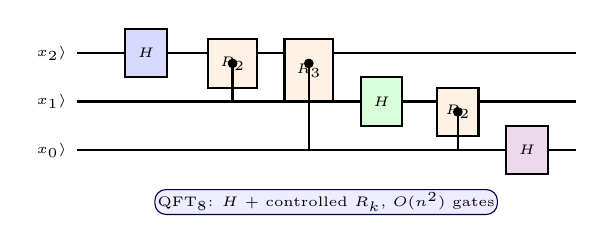
\begin{tikzpicture}[scale=0.88,font=\footnotesize]
  \draw[thick] (0,1.4)--(7.2,1.4);
  \draw[thick] (0,0.7)--(7.2,0.7);
  \draw[thick] (0,0)--(7.2,0);
  \node[left, font=\tiny] at (0,1.4) {$\lvert x_2\rangle$};
  \node[left, font=\tiny] at (0,0.7) {$\lvert x_1\rangle$};
  \node[left, font=\tiny] at (0,0) {$\lvert x_0\rangle$};
  % 3-qubit QFT
  \draw[fill=blue!15, thick] (0.7,1.05) rectangle (1.3,1.75) node[midway, font=\tiny] {$H$};
  \draw[fill=orange!10, thick] (1.9,0.9) rectangle (2.6,1.6) node[midway, font=\tiny] {$R_2$};
  \draw[fill=orange!10, thick] (3.0,0.7) rectangle (3.7,1.6) node[midway, font=\tiny] {$R_3$};
  \fill (2.25,1.25) circle (2pt); \draw[thick] (2.25,1.25)--(2.25,0.7);
  \fill (3.35,1.25) circle (2pt); \draw[thick] (3.35,1.25)--(3.35,0);
  \draw[fill=green!15, thick] (4.1,0.35) rectangle (4.7,1.05) node[midway, font=\tiny] {$H$};
  \draw[fill=orange!10, thick] (5.2,0.2) rectangle (5.8,0.9) node[midway, font=\tiny] {$R_2$};
  \fill (5.5,0.55) circle (2pt); \draw[thick] (5.5,0.55)--(5.5,0);
  \draw[fill=violet!15, thick] (6.2,-0.35) rectangle (6.8,0.35) node[midway, font=\tiny] {$H$};
  \node[font=\tiny, fill=blue!7, draw=blue!30!black, rounded corners, inner sep=1pt] at (3.6,-0.75) {QFT$_8$: $H$ + controlled $R_k$, $O(n^2)$ gates};
\end{tikzpicture}
\end{center}

\begin{center}
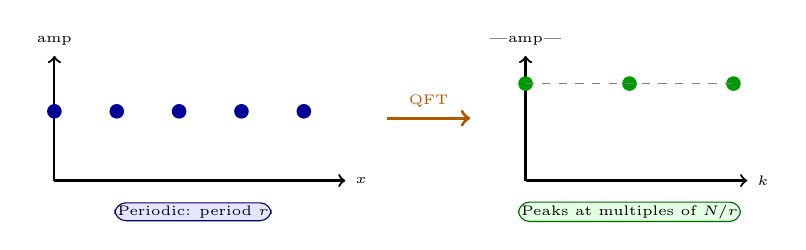
\begin{tikzpicture}[scale=0.88,font=\footnotesize]
  % Periodic signal -> peaks
  \draw[->, thick] (0,0)--(4.2,0) node[right, font=\tiny] {$x$};
  \draw[->, thick] (0,0)--(0,1.8) node[above, font=\tiny] {amp};
  \foreach \x in {0,0.9,1.8,2.7,3.6} \fill[blue!60!black] (\x,1.0) circle (3pt);
  \node[font=\tiny, fill=blue!10, draw=blue!40!black, rounded corners, inner sep=1pt] at (2.0,-0.45) {Periodic: period $r$};
  \draw[->, very thick, orange!70!black] (4.8,0.9)--(6.0,0.9) node[midway, above, font=\tiny] {QFT};
  \begin{scope}[shift={(6.8,0)}]
    \draw[->, thick] (0,0)--(3.2,0) node[right, font=\tiny] {$k$};
    \draw[->, thick] (0,0)--(0,1.8) node[above, font=\tiny] {|amp|};
    \foreach \x in {0,1.5,3.0} \fill[green!60!black] (\x,1.4) circle (3pt);
    \draw[dashed, gray] (0,1.4)--(3.0,1.4);
    \node[font=\tiny, fill=green!10, draw=green!40!black, rounded corners, inner sep=1pt] at (1.5,-0.45) {Peaks at multiples of $N/r$};
  \end{scope}
\end{tikzpicture}
\end{center}

\section{Shor's Period-Finding Circuit}
\begin{enumerate}[nosep,left=12pt]
\item Prepare $\tfrac1{\sqrt Q}\sum_{x=0}^{Q-1}\lvert x\rangle\lvert0\rangle$ with $Q=2^n\approx N^2$.
\item Apply $U_f:\lvert x\rangle\lvert0\rangle\mapsto\lvert x\rangle\lvert a^x\bmod N\rangle$.
\item Measure second register (optional) giving periodic state $\tfrac1{\sqrt m}\sum_j\lvert x_0+jr\rangle$.
\item QFT on first register, measure to get $k\approx cQ/r$, then continued fractions recover $r$.
\end{enumerate}

\begin{theorem}[Shor 1994]
Period finding succeeds with probability $\Omega(1)$ using $O(n^2)$ quantum gates. Classical factoring best known is $\exp(O(n^{1/3}))$. Factoring $N$ reduces to period finding with one extra gcd step, so factoring is in BQP.
\end{theorem}

\begin{center}
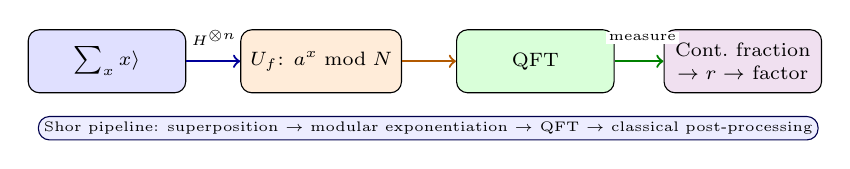
\begin{tikzpicture}[scale=0.85,font=\footnotesize]
  \node[draw, fill=blue!12, rounded corners, minimum width=2.0cm, minimum height=0.8cm, font=\scriptsize] (sup) at (0,0) {$\sum_x\lvert x\rangle$};
  \node[draw, fill=orange!15, rounded corners, minimum width=2.0cm, minimum height=0.8cm, font=\scriptsize] (uf) at (3.2,0) {$U_f$: $a^x\bmod N$};
  \node[draw, fill=green!15, rounded corners, minimum width=2.0cm, minimum height=0.8cm, font=\scriptsize] (qft) at (6.4,0) {QFT};
  \node[draw, fill=violet!12, rounded corners, minimum width=2.0cm, minimum height=0.8cm, font=\scriptsize, align=center] (cf) at (9.5,0) {Cont.\ fraction\\$\to r\to$ factor};
  \draw[->, thick, blue!60!black] (sup)--(uf);
  \draw[->, thick, orange!70!black] (uf)--(qft);
  \draw[->, thick, green!50!black] (qft)--(cf);
  \node[font=\tiny, fill=white, inner sep=1pt] at (1.6,0.35) {$H^{\otimes n}$};
  \node[font=\tiny, fill=white, inner sep=1pt] at (8.0,0.35) {measure};
  \node[fill=blue!7, draw=blue!30!black, rounded corners, inner sep=2pt, font=\tiny] at (4.8,-1.0) {Shor pipeline: superposition $\to$ modular exponentiation $\to$ QFT $\to$ classical post-processing};
\end{tikzpicture}
\end{center}

\section{Example: Factoring 15}
Pick $a=7$, $N=15$. Powers $7^x\bmod15$: $1,7,4,13,1,\dots$ period $r=4$ (even). $a^{r/2}=7^2=49\equiv4\bmod15$, $\gcd(4-1,15)=3$, $\gcd(4+1,15)=5$. A $Q=16$ QFT on a period-$4$ signal gives peaks at $k=0,4,8,12$; measurement yields $cQ/r$ and $r=4$ via continued fractions on $k/Q$.


\section{Continued Fractions and Classical Post-Processing}
Measurement yields integer $k$ with $|k/Q-c/r|\le1/2Q$ for some $c$. The fraction $k/Q$ approximates $c/r$. Expanding $k/Q$ as a continued fraction lists convergents $p_j/q_j$; the denominator $q_j\approx r$ when $Q\ge N^2$. Testing $a^{q_j}\equiv1\bmod N$ recovers $r$. If $c$ and $r$ share a factor, the convergent gives a divisor of $r$; retry with a new $k$ or take $\mathrm{lcm}$ of several candidates.

\begin{example}[Failure modes and retry]
Take $N=21$, $a=2$, true $r=6$. If measurement gives $k=11$, $Q=64$, then $k/Q=0.1719\approx1/6=0.1667$ and continued fraction $11/64=[0;5,1,4,2]$ yields convergents $1/5,1/6$ --- success. If $k=32$, then $k/Q=1/2$ gives $r=2$ (a divisor); $a^2=4\neq1\bmod21$, so double to $r=6$ after checking multiples.
\end{example}


\section{Shor vs.\ Grover: Exponential vs.\ Quadratic}
Shor achieves superpolynomial speedup because factoring has hidden periodic structure that QFT exposes. Grover's problem is structureless, so only quadratic is possible (and optimal). This dichotomy guides algorithm design: look for hidden subgroup, hidden shift, or algebraic structure for exponential advantage; use amplitude amplification for generic search and optimization where only quadratic is expected.

\section{Resource Estimates}
Modular exponentiation dominates: $O(n^3)$ gates naively, $O(n^2\log n)$ with FFT multiplication. For RSA-2048 ($n=2048$), Shor needs $\sim4000$ logical qubits and $\sim10^9$ Toffoli gates. With distance $d=27$ surface code ($p=10^{-3}$), that's $\sim10^6$ physical qubits and hours of runtime --- beyond NISQ but within fault-tolerant roadmaps at $10^{-4}$ error rates.


\section{Historical Impact and Cryptography}
Shor's 1994 result triggered post-quantum cryptography. RSA, Diffie--Hellman and ECDSA all reduce to hidden subgroup over abelian groups, thus fall to Shor. NIST's 2024 standards (Kyber for KEM, Dilithium for signatures) are lattice-based, conjectured resistant because the hidden subgroup structure is non-abelian or absent. Migrating the internet to PQC is underway before large fault-tolerant machines arrive.

\section{Python: QFT and Period Finding}

\begin{lstlisting}[language=Python]
import numpy as np

def qft_matrix(N):
    w = np.exp(2j*np.pi/N)
    j, k = np.meshgrid(np.arange(N), np.arange(N), indexing='ij')
    return (w**(j*k))/np.sqrt(N)

def qft_circuit_unitary(n):
    return qft_matrix(2**n)

# Verify unitary for n=3
for n in [1,2,3]:
    U = qft_circuit_unitary(n)
    err = np.linalg.norm(U @ U.conj().T - np.eye(2**n))
    print(f"n={n} QFT unitary error {err:.2e}")

# Period finding demo: N=15, a=7, Q=16
N_mod, a, Q = 15, 7, 16
f = [pow(a, x, N_mod) for x in range(Q)]
print("f(x)=7^x mod15:", f)  # period 4
# Simulate: periodic state with period 4 -> QFT peaks
ps = np.zeros(Q, dtype=complex)
for x in range(0, Q, 4):  # period-4 comb
    ps[x] = 1
ps /= np.linalg.norm(ps)
amps = qft_matrix(Q) @ ps
probs = np.abs(amps)**2
print("QFT peaks at k:", np.where(probs > 0.1)[0])
\end{lstlisting}

\begin{lstlisting}[language=Python]
# Full Shor factoring for N=15 (classical post-processing)
import math, random

def shor_factor(N, a, Q=64):
    # Quantum part: estimate period r via QFT peaks (simulated)
    # Find r = order of a mod N classically for demo
    r = 1
    while pow(a, r, N) != 1:
        r += 1
        if r > N: return None
    if r % 2 == 1: return None
    ar2 = pow(a, r//2, N)
    if ar2 == N-1: return None
    f1 = math.gcd(ar2-1, N)
    f2 = math.gcd(ar2+1, N)
    return r, f1, f2

for a in [2,7,8,11]:
    res = shor_factor(15, a)
    print(f"a={a} -> {res}")

# Continued fraction to recover r from k/Q
from fractions import Fraction
k, Q = 48, 64  # example measurement k=48
frac = Fraction(k, Q).limit_denominator(15)
print(f"k/Q={k}/{Q} -> {frac} => r={frac.denominator}")
\end{lstlisting}


\section{From Period to Factor: Number Theory Step}
Given even $r$ with $a^{r/2}\neq-1\bmod N$, write $a^r-1=(a^{r/2}-1)(a^{r/2}+1)\equiv0\bmod N$. So $N$ divides the product but neither factor alone, hence each shares a non-trivial gcd with $N$. The number-theoretic lemma: for random $a$ coprime to $N=pq$ with distinct odd primes, $\Pr[r\text{ even and }a^{r/2}\neq-1]\ge1/2$. Thus a few random $a$'s succeed with high probability. The full factoring algorithm is Las Vegas: quantum period finding plus classical gcd, poly time overall.

\begin{remark}
Shor also solves discrete log $g^x=h$ by two-dimensional period finding, breaking Diffie--Hellman and elliptic-curve cryptography. Post-quantum candidates (lattices, codes, isogenies) resist known period-finding attacks because their structure is not abelian hidden subgroup.
\end{remark}


\begin{remark}[Continued fractions]
Dirichlet: if $|k/Q-c/r|\le1/2Q$ and $Q\ge N^2$, then $c/r$ is a convergent of $k/Q$. Denominators grow exponentially, so $O(\log Q)$ convergents suffice. Testing each $q_j$ via $a^{q_j}\equiv1$ finds $r$ or a divisor.
\end{remark}

\begin{example}[Coprime failure]
If $\gcd(c,r)=d>1$, convergent gives $r/d$. Fresh $k$ yields another divisor; $\mathrm{lcm}$ recovers $r$. Failure per shot $\le1/\log r$, so $O(\log N)$ repetitions boost success to $1-1/\mathrm{poly}(N)$.
\end{example}

\begin{remark}[Modular exponentiation]
Repeated squaring computes $a^x\bmod N$ with $O(n)$ multiplications, each $O(n^2)$ naively or $O(n\log n)$ with FFT. Quantumly a permutation implemented reversibly with $O(n^3)$ Toffoli gates; windowed arithmetic reduces count below $10^9$ for $n=2048$.
\end{remark}

\section{Exercises}
\begin{exercise}
Prove QFT is unitary and that QFT$_2=H$. How many $R_k$ gates does QFT$_{2^n}$ use? Show an $O(n\log n)$ approximate QFT drops small-angle $R_k$ with error $\le\epsilon$.
\end{exercise}
\begin{exercise}
For $f(x)=7^x\bmod15$ with $Q=16$, write the state before QFT after measuring $f=4$ in the second register. Compute QFT output probabilities and list possible $k$ values.
\end{exercise}
\begin{exercise}
Given measured $k=6$, $Q=16$, use continued fractions on $k/Q$ to find candidate $r$. Which convergents give the correct period $r=4$? What if $k=12$?
\end{exercise}
\begin{exercise}
Show if $r$ is odd or $a^{r/2}\equiv-1\bmod N$, Shor's gcd step fails. Estimate the probability a random $a$ coprime to $N=pq$ yields a useful $r$ (at least $1/2$ for distinct odd primes).
\end{exercise}
\begin{exercise}
Implement modular exponentiation $U_f$ for $N=21$, $a=2$ as a permutation matrix on $n=6$ qubits and verify its action on $\lvert x\rangle\lvert0\rangle$.
\end{exercise}
